\chapter{Giới thiệu}
\label{chap:intro}

\section{Động lực nghiên cứu}
Bệnh Alzheimer (Alzheimer's disease -- AD) là dạng sa sút trí tuệ thường gặp nhất. Bệnh tiến triển theo thời gian, ảnh hưởng đến trí nhớ, tư duy và khả năng sinh hoạt độc lập \cite{cdc2024alzheimers}. Ở người có suy giảm nhận thức nhẹ (Mild Cognitive Impairment -- MCI), chức năng nhận thức đã suy giảm nhưng khả năng tự chủ trong sinh hoạt thường ngày còn được duy trì. Việc thực hiện những hoạt động phức tạp có thể khó khăn hơn \cite{jack2018niaaa}. Diễn tiến ở nhóm này khác nhau giữa các cá thể: một số người tiến triển thành sa sút trí tuệ, trong khi những người khác có thể ổn định hoặc cải thiện \cite{petersen2018mci}. Từ sự khác biệt đó, khóa luận đặt câu hỏi: \emph{Có thể dùng lịch sử thăm khám để xếp hạng nguy cơ tiến triển của từng người mắc MCI hay không?}

Một ảnh MRI tại một thời điểm cho biết cấu trúc não khi chụp. Để quan sát trực tiếp sự thay đổi của một cấu trúc ở cùng cá thể, cần so sánh các lần chụp. Chẳng hạn, Dong và cộng sự sử dụng các cặp MRI của cùng người tham gia để định lượng biến đổi theo thời gian ở vùng hồi hải mã \cite{dong2021deepatrophy}. Trong nhóm nghiên cứu của khóa luận, khoảng cách giữa hai lần chụp liên tiếp thay đổi theo từng người (Bảng~\ref{tab:baseline-characteristics}). Vì vậy, mô hình tiếp nhận cả thứ tự và khoảng cách thực tế giữa các lần chụp, theo cách tiếp cận của mạng bộ nhớ dài ngắn hạn có xét thời gian (T-LSTM) dành cho hồ sơ bệnh nhân có khoảng quan sát không đều \cite{baytas2017patient}.

Bên cạnh thời gian theo dõi, khóa luận khai thác ba nguồn thông tin:
\begin{enumerate}
\item \emph{Ảnh cộng hưởng từ cấu trúc 3D (MRI)} cung cấp thông tin giải phẫu về các biến đổi như teo hồi hải mã và giãn não thất \cite{weiner2015impact}.
\item \emph{Radiomics} lượng hóa hình dạng, phân bố cường độ và kết cấu bên trong vùng ảnh được phân tích \cite{vangriethuysen2017computational}.
\item \emph{Dữ liệu lâm sàng} cung cấp điểm MMSE để đánh giá nhận thức và điểm CDR để đánh giá mức độ suy giảm nhận thức và chức năng sinh hoạt \cite{folstein1975mmse,morris1993cdr}.
\end{enumerate}
Mặc dù ba nguồn dữ liệu trên có tiềm năng bổ khuyết mạnh mẽ, việc hợp nhất chúng lại đặt ra thách thức lớn do sự khác biệt sâu sắc về bản chất toán học, kích thước đặc trưng và độ nhiễu đo lường.

Aghajanian và cộng sự (2025) kết hợp mạng nơ-ron tích chập (CNN), phân tích thành phần chính (PCA), T-LSTM và cơ chế chú ý (attention) để tổng hợp chuỗi MRI dọc và ước lượng nguy cơ theo mô hình Cox \cite{aghajanian2025longitudinal}. Trong Bảng~2 của công trình này, khi thêm radiomics chất xám vào mô hình T-LSTM có attention, C-index trung bình chuyển từ 0.85 xuống 0.84 trên tập xác thực và từ 0.91 xuống 0.90 trên tập kiểm tra. Các tác giả chọn cấu hình không dùng radiomics cho mô hình cuối \cite{aghajanian2025longitudinal}. Từ kết quả đó, khóa luận khảo sát liệu cách hợp nhất đặc trưng có ảnh hưởng đến giá trị tiên lượng của radiomics hay không.

Khóa luận kế thừa quy trình của Aghajanian và cộng sự làm đối chứng cơ sở, đồng thời mô hình hóa tường minh các tương tác song tuyến giữa từng cặp phương thức. Ba nguồn dữ liệu MRI (M), radiomics (R) và lâm sàng (C) tạo thành ba cặp tương tác: MRI--Radiomics (MR), MRI--Lâm sàng (MC) và Radiomics--Lâm sàng (RC). Để giảm số tham số so với phép tích ngoài đầy đủ, tôi áp dụng phân rã tensor Canonical Polyadic (CP) hạng thấp \cite{kolda2009tensor,liu2018lowrank}, kết hợp với cơ chế truyền phần dư có cổng. Vì radiomics được trích từ chính ảnh MRI, tôi chọn MRI làm đầu vào chung cho hai cặp trong kiến trúc \textbf{RC-Free Pairwise Fusion (RC-Free)}. Kiến trúc này giữ MR và MC, bỏ tương tác trực tiếp RC. Ảnh hưởng của lựa chọn đó được kiểm tra bằng cách so sánh các cấu trúc tương tác ở Mục~\ref{sec:new-topology}.

\section{Phát biểu bài toán}
Đề tài \emph{Longitudinal Learning with Tensor Fusion for Predicting Progression of Alzheimer's Disease} xây dựng mô hình xếp hạng nguy cơ tiến triển cho nhóm người mắc MCI trong bộ dữ liệu Alzheimer's Disease Neuroimaging Initiative (ADNI) \cite{weiner2015impact}. Quần thể nghiên cứu gồm 359 người tham gia có đủ ba lần chụp MRI trong vòng 18 tháng kể từ lần khám ban đầu. Mỗi lần chụp được liên kết đồng bộ với các đặc trưng radiomics và các bài kiểm tra lâm sàng tương ứng. Ba mốc thời gian chụp $s_1<s_2<s_3=p\leq L$ tạo thành một chuỗi quan sát dọc có các khoảng cách thời gian biến thiên thực tế. Mục tiêu cốt lõi của mô hình là từ chuỗi quan sát đa phương thức này, ước lượng cho mỗi cá thể một điểm số log-nguy cơ $\eta_i\in\mathbb R$ để xếp hạng thứ tự rủi ro suy giảm nhận thức trong tương lai.

\begin{figure}[H]
\centering
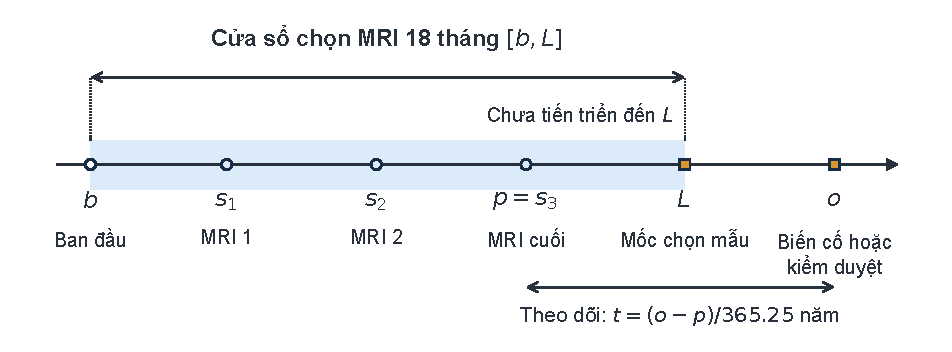
\includegraphics[width=\textwidth]{image/mci-progression-timeline.pdf}
\caption{Bài toán dự đoán tiến triển MCI theo thời gian}
\label{fig:problem-timeline}
\end{figure}

Hình~\ref{fig:problem-timeline} trực quan hóa tiến trình theo dõi và làm rõ mối quan hệ giữa ngày chụp MRI cuối cùng $p$ với mốc chọn mẫu $L$ (được ấn định bằng ngày khám ban đầu cộng 18 tháng lịch). Để lượng hóa trạng thái nhận thức và năng lực tự chủ của người bệnh, nghiên cứu sử dụng hai thang đo tiêu chuẩn:
\begin{enumerate}
\item \emph{MMSE (Mini-Mental State Examination)}: Thang điểm đánh giá nhận thức tổng quát từ 0 đến 30, trong đó điểm số càng thấp phản ánh mức độ sa sút nhận thức càng nghiêm trọng \cite{folstein1975mmse}.
\item \emph{CDR-global (Clinical Dementia Rating toàn cục)}: Các mức 0, 0.5, 1, 2 và 3 lần lượt tương ứng với bình thường, sa sút trí tuệ rất nhẹ, nhẹ, vừa và nặng theo bảng phân mức của đơn vị phát triển thang đo \cite{morris1993cdr,knightcdrscoring}.
\end{enumerate}

Theo tiêu chí nghiên cứu của Aghajanian và cộng sự \cite{aghajanian2025longitudinal}, khóa luận ghi nhận biến cố tiến triển ở lần khám đầu tiên sau mốc chọn mẫu $L$ có điểm MMSE $<24$ hoặc CDR-global $\geq1$. Đây là biến cố xác định bằng điểm số. Những người tham gia kết thúc theo dõi mà chưa từng ghi nhận biến cố được xem là \emph{kiểm duyệt phải} (right-censored) tại lần khám hợp lệ cuối cùng. Phân tích sống còn khai thác đồng thời cả thời gian theo dõi lẫn thông tin kiểm duyệt này.

Về mặt thiết kế phương pháp luận, khóa luận tính thời gian sống còn đến biến cố hoặc kiểm duyệt bắt đầu từ ngày chụp MRI cuối cùng $p$, trong khi tiêu chí chọn mẫu đòi hỏi người tham gia phải duy trì tình trạng chưa tiến triển cho đến mốc $L$. Chẳng hạn, với một người có lần MRI cuối ở tháng thứ 12 và mốc chọn mẫu ở tháng thứ 18, khoảng thời gian 6 tháng giữa $p$ và $L$ được tính vào thời gian theo dõi nhưng mặc nhiên không có biến cố. Do đó, đối tượng nghiên cứu được xác định chặt chẽ là nhóm bệnh nhân hồi cứu thỏa mãn điều kiện tại $L$. Khía cạnh phương pháp luận này, cùng nguy cơ sai lệch thời gian bất tử \cite{suissa2008immortal} khi diễn giải mô hình như một công cụ dự báo tại $p$, được trình bày và thảo luận cụ thể tại Mục~\ref{sec:study-design} và Mục~\ref{sec:study-limitations}.

\section{Thách thức và phạm vi nghiên cứu}
Việc xây dựng một mô hình học sâu sống còn trên dữ liệu y tế dọc đa phương thức đối mặt với ba thách thức phương pháp luận trung tâm:

Thứ nhất là \emph{đánh đổi giữa khả năng biểu diễn tương tác và số tham số cần ước lượng}. Phép ghép nối vectơ đặt các đặc trưng cạnh nhau để các tầng sau học mối liên hệ giữa chúng. Phép tích ngoài biểu diễn tường minh các tích chéo giữa các phương thức. Khi dùng một lớp tuyến tính đầy đủ để chiếu biểu diễn này, số trọng số tăng theo tích các kích thước đầu vào và đầu ra \cite{zadeh2017tensor,liu2018lowrank}. Với cỡ mẫu của khóa luận, đây là một nguy cơ quá khớp cần khảo sát. Phân rã CP giảm số trọng số bằng cách áp đặt cấu trúc hạng thấp \cite{kolda2009tensor,liu2018lowrank}. Ảnh hưởng của ràng buộc này đến năng lực phân biệt của mô hình cần được kiểm chứng bằng thực nghiệm.

Thứ hai là \emph{khả năng dư thừa thông tin giữa các nguồn dữ liệu}. Ảnh MRI và đặc trưng radiomics bắt nguồn từ cùng một thể tích ảnh gốc, còn các thang đo lâm sàng ở lần khám sau được dùng để xác định biến cố. Vì vậy, khóa luận kiểm tra bằng thực nghiệm liệu có cần giữ cả ba cặp tương tác hay chỉ cần hai cặp có chung đầu vào MRI. Hiệu quả dự báo của từng cấu hình được đánh giá qua so sánh loại bỏ thành phần.

Thứ ba là \emph{sự phức tạp của cấu trúc dữ liệu thời gian không đều và mục tiêu tối ưu hóa sống còn}. Mô hình phải xử lý đồng thời chuỗi quan sát có khoảng cách thời gian bất quy tắc bằng T-LSTM và attention, đồng thời tối ưu hóa hàm mất mát Cox trên các lô nhỏ mà không làm mất tính ổn định số học.

Để giải quyết thấu đáo ba thách thức trên, phạm vi nghiên cứu của khóa luận tập trung khảo sát có hệ thống: cách biểu diễn tương tác song tuyến qua tích ngoài, mức độ tinh giản tham số nhờ phân rã CP, và ảnh hưởng của việc lược bỏ cặp tương tác trong cấu trúc RC-Free. Mọi so sánh đối chứng đều được thực hiện nghiêm ngặt trên cùng một cách chia dữ liệu, sử dụng thống nhất ba mã khởi tạo ngẫu nhiên (seed) và đánh giá qua chỉ số đồng thuận (C-index), diện tích dưới đường cong ROC phụ thuộc thời gian (IPCW-ROC) cùng đường cong sống còn Kaplan--Meier.

\section{Câu hỏi nghiên cứu}
Nhằm định hướng cho toàn bộ các thực nghiệm đối chứng trong khóa luận, tôi xây dựng năm câu hỏi nghiên cứu cụ thể được tổng hợp tại Bảng~\ref{tab:rq}. Trong đó, RQ1 và RQ2 khảo sát vai trò của dữ liệu dọc và tính bổ khuyết của các nguồn dữ liệu đầu vào; RQ3 tập trung đối chiếu bản chất của phép hợp nhất tích ngoài so với ghép nối; trong khi RQ4 và RQ5 thẩm định hiệu quả giảm tham số của phân rã CP và tính ưu việt của cấu trúc tinh giản RC-Free.

\begin{table}[H]
\centering\small
\caption[Các câu hỏi nghiên cứu và phương pháp kiểm chứng]{Các câu hỏi nghiên cứu và phương pháp kiểm chứng.}
\label{tab:rq}
\setlength{\tabcolsep}{6pt}
\renewcommand{\arraystretch}{1.12}
\begin{tabularx}{\textwidth}{@{}Y Y@{}}
\toprule
\textbf{Câu hỏi nghiên cứu} & \textbf{Phương pháp kiểm chứng} \\
\midrule
\textbf{RQ1.} MRI ở nhiều thời điểm có mang lại khả năng phân biệt nguy cơ cao hơn so với chỉ dùng MRI cuối cùng không? & Đối chiếu mô hình \textit{MRI cuối} với \textit{MRI dọc và T-LSTM} cùng \textit{MRI dọc, T-LSTM và attention} để khảo sát vai trò của thông tin theo thời gian. \\
\addlinespace
\textbf{RQ2.} Bổ sung radiomics và lâm sàng có cải thiện khả năng phân biệt nguy cơ so với chỉ dùng MRI không? & Đối chiếu \textit{MRI dọc, T-LSTM và attention} với \textit{Ghép nối ba nguồn (thăm dò)} sử dụng cả ba nguồn dữ liệu. \\
\addlinespace
\textbf{RQ3.} Tương tác theo cặp có hiệu quả hơn ghép nối đặc trưng không? & So sánh ghép nối và tích ngoài qua ba lần chạy, dùng cùng cách huấn luyện và cùng trọng số ban đầu cho các phần chung. \\
\addlinespace
\textbf{RQ4.} CP giảm bao nhiêu tham số của lớp tương tác và ảnh hưởng thế nào đến C-index? & So sánh Full Outer-Product và Full CP Pairwise về C-index và số tham số ở từng phạm vi. \\
\addlinespace
\textbf{RQ5.} Có thể bỏ một số cặp tương tác và nhánh truyền mà vẫn duy trì khả năng phân biệt nguy cơ không? & Thực nghiệm loại bỏ thành phần đối chiếu 7 cấu trúc tương tác (gồm các biến thể 1 cặp, 2 cặp như RC-Free, MR-Free, MC-Free và Full CP) để đánh giá cấu trúc tối ưu. \\
\bottomrule
\end{tabularx}
\end{table}

\FloatBarrier
\Needspace{11\baselineskip}
\section{Đóng góp của khóa luận}
Khóa luận mang lại ba đóng góp phương pháp luận và thực nghiệm chính:
\begin{enumerate}
\item \emph{Xây dựng mô hình học sâu sống còn đa phương thức dọc toàn diện}: Đề xuất một kiến trúc hoàn chỉnh tích hợp đồng thời ba nguồn dữ liệu — ảnh MRI cấu trúc 3D, đặc trưng Radiomics định lượng và dữ liệu lâm sàng MMSE/CDR — qua ba mốc thăm khám dọc. Mô hình kết hợp bộ mã hóa ResNet-18 3D tiền huấn luyện trên dữ liệu y tế \cite{chen2019med3d}, mạng T-LSTM xử lý khoảng cách thời gian bất quy tắc \cite{baytas2017patient}, cơ chế attention học trọng số thăm khám then chốt và đầu ra nguy cơ Cox bán tham số.
\item \emph{Thiết kế cơ chế truyền phần dư có cổng và kiến trúc tinh gọn RC-Free}: Phát triển cơ chế kết nối phần dư có cổng điều tiết động (gated residual routing) giúp bảo toàn nguyên vẹn đường truyền gốc của từng phương thức, đồng thời xem thông tin tương tác như phần bổ chính có kiểm soát. Chọn MRI làm đầu vào chung cho hai cặp tương tác, tôi đề xuất cấu trúc \textbf{RC-Free} — lược bỏ cặp tương tác trực tiếp Radiomics--Lâm sàng (RC), tập trung tối đa vào hai tương tác cốt lõi xoay quanh MRI là MRI--Radiomics (MR) và MRI--Lâm sàng (MC).
\item \emph{Lượng hóa hiệu quả giảm tải tham số và năng lực phân tầng nguy cơ}: Thông qua phân rã tensor CP, mô hình cắt giảm tới \textbf{98.38\%} số tham số ở các lớp tương tác đầu và tiết kiệm \textbf{15460 tham số} toàn mạng khi loại bỏ cặp RC. Trên cùng một quy trình chia dữ liệu độc lập và đánh giá qua ba lần khởi tạo, RC-Free đạt C-index xác thực trung bình cao nhất trong bảy cấu trúc tương tác theo cặp (\textbf{0.8347}), phân tầng rõ nét hai nhóm nguy cơ trên đường cong Kaplan--Meier ($p=0.0134$ trên tập xác thực và $p<0.001$ trên tập kiểm tra hậu nghiệm), theo các kết quả của khóa luận ở Bảng~\ref{tab:interaction-parameters}, Bảng~\ref{tab:new-topology} và Bảng~\ref{tab:km-statistics}.
\end{enumerate}
